\documentclass{article}

\title{Inverses in Higher Categories}
\author{Alex Rice}

\usepackage{verbatim}
\usepackage[nomarginpar]{geometry}
\usepackage{amsmath}
\usepackage{amssymb}
\usepackage{amsfonts}
\usepackage{mathtools}
\usepackage{amsthm}
\usepackage{cleveref}
\usepackage{tikz}
\usepackage{listings}

\lstset{basicstyle=\ttfamily,
mathescape=true}

\usetikzlibrary{positioning}

\newtheorem{theorem}{Theorem}
\newtheorem{prop}{Proposition}
\newtheorem{cor}{Corollary}
\newtheorem{lemma}{Lemma}
\theoremstyle{definition}
\newtheorem{definition}{Definition}
\newtheorem{remark}{Remark}
\newtheoremstyle{examplestyle}% name
{20pt}% Space above
{20pt}% Space below
{\rmfamily}% Body font
{}%Indent amount (empty = no indent, \parindent = para indent)
{\bfseries}% Thm head font
{.}% Punctuation after thm head
{ }% Space after thm head: " " = normal interword space;
% \newline = linebreak
{}% Thm head spec
\theoremstyle{examplestyle}
\newtheorem{example}{Example}

\DeclareMathOperator{\id}{id}

\newcommand{\linv}[1]{{}^\star\!#1}
\newcommand{\rinv}[1]{#1^\star}


\begin{document}
\maketitle

\begin{definition}
  The globe category \(\mathbb{G}\) is the category where the objects are the natural numbers and morphisms are generated by
  \begin{align*}
    &\sigma_n : n \to n+1\\
    &\tau_n : n \to n+1
  \end{align*}
  subject to the conditions
  \begin{align*}
    \sigma \circ \sigma &= \tau \circ \sigma\\
    \sigma \circ \tau &= \tau \circ \tau
  \end{align*}
\end{definition}

\begin{definition}
  A globular set \(G\) is a presheaf of \(\mathbb{G}\). We refer to \(G(n)\) as the set of \(n\)-cells and for two \(n\)-cells \(x\) and \(y\) we write \(f: x \to y\) to mean that \(f\) is an \((n+1)\)-cell and
  \begin{align*}
    G(\sigma_n)(f) &= x\\
    G(\tau_n)(f) &= y
  \end{align*}
  where we call \(x\) the source of \(f\) and \(y\) the target of \(f\).
\end{definition}

\begin{definition}
  A globular set with identities and composition is a globular set \(G\) with the following:
  \begin{itemize}
  \item For each \(n\)-cell \(x\), there is an \((n+1)\)-cell, \(\id_x\).
  \item Inductively define composition as follows:
    \begin{itemize}
    \item Given \(n\)-cells \(f: x \to y\) and \(g: y \to z\) there is
      an \(n\)-cell \(g \circ_0 f: x \to z\).
    \item Given \(\alpha: f \to g\) and \(\beta: h \to j\), where the composites \(f \circ_n h\) and \(g \circ_n j\) are well defined, there is a morphism \(\alpha \circ_{n+1} \beta: (f \circ_n h) \to (g \circ_n j)\)
    \end{itemize}
  \end{itemize}
  \(\circ\) will be used to mean \(\circ_0\).
\end{definition}

\begin{definition}
  Given a globular set \(G\) with identities and composition, we define the collection of \emph{bi-invertible} cells of \(G\) coinductively as follows: For \(n > 0\), an \(n\)-cell \(f: x \to y\) is \emph{bi-invertible} if:
  \begin{itemize}
  \item There exists an \(n\)-cell \(\rinv f: y \to x\).
  \item There exists an \(n\)-cell \(\linv f: y \to x\).
  \item There exists an \((n+1)\)-cell \(f_R: f \circ \rinv f \to \id_y\).
  \item There exists an \((n+1)\)-cell \(f_L: \linv f \circ f \to \id_x\).
  \item \(f_R\) is \emph{bi-invertible}.
  \item \(f_L\) is \emph{bi-invertible}.
  \end{itemize}
\end{definition}

\begin{remark}
  It can be useful to think of \emph{bi-invertibility} as a functional datatype which encodes a ``proof'' of bi-invertibility. This datatype will clearly be coinductive. We can define this datatype (in a pseudo-Agda syntax) as follows.

  \begin{lstlisting}
    codata BiInvertible (f: x $\to$ y) where
      $\rinv {\mathtt{f}}$: y $\to$ x,
      $\linv {\mathtt{f}}$: y $\to$ x,
      f_R: $\mathtt f \circ \rinv {\mathtt {f}} \to \mathtt{id}_{\mathtt y}$,
      f_L: $\linv {\mathtt {f}} \circ {\mathtt {f}} \to \mathtt{id}_{\mathtt y}$,
      f_RProof: BiInvertible f_R,
      f_LProof: BiInvertible f_L
  \end{lstlisting}
\end{remark}

\begin{definition}
  \label{def:higher-cat}
  We define an infinity category as a globular set with identities and composition that respects the graphical calculus in the following way. We may draw a diagram with nodes, lines, and areas where areas will represent \(n\)-cells, lines represent \((n+1)\)-cells, and nodes represent \((n+2)\)-cells. Then for any planar isotopy of this diagram there is an \((n+3)\)-cell from source of the isotopy to the target. Further, this cell is \emph{bi-invertible}. Further we assume the existence of the following morphisms.
  \begin{itemize}
  \item For \(n>0\) and each \(n\)-cell \(f: x \to y\), there are \(n+1\)-cells, known as unitors, \(\lambda_f: \id_y \circ f \to f\) and \(\rho_f: f \circ \id_x \to f\).
  \item Given \(f,g,h,j\), \(n>1\)-cells composition defined, we have an associator \(a_{f,g,h,j} : (f \circ g) \circ (h \circ j) \to (f \circ (g \circ h) \circ j)\).
  \item For compatible morphisms \(f,g,h,j\), we have an interchanger \(i_{f,g,h,j}(f \circ_n g) \circ (h \circ_n j) \to (f \circ h) \circ_n (g \circ j)\).
  \item For suitable \(f,g\) and \(n > 1\), there is a cell \(\id_f \circ_{n+1} \id_g \to \id_{f \circ_n g}\)
  \end{itemize}
  These are all \emph{bi-invertible}.
\end{definition}

We prove some helpful facts about \emph{bi-invertible} morphisms in higher categories.

\begin{lemma}
  \label{lem:identity}
  Any identity morphism is \emph{bi-invertible}.
\end{lemma}

\begin{proof}
  Let \(x\) be any cell. Take \(\rinv {\id_x} = \linv {\id_x} = \id_x\) and \((\id_x)_R = (\id_x)_L = \lambda_{id_x}\). By assumption, \(\lambda_{id_x}\) is \emph{bi-invertible}. Hence \(\id_x\) is \emph{bi-invertible}.
\end{proof}

\begin{theorem}[Composition of \emph{Bi-invertible} Morphisms]
  For any \(n \in \mathbb{N}\) and \emph{bi-invertible} cells \(f,g\), \(f \circ_n g\) is \emph{bi-invertible} if it is well defined.
\end{theorem}
\begin{proof}
  The proof has a nested coinductive proof. We wish to describe a procedure taking the data that a pair of compatible cells are \emph{bi-invertible} cells to a proof of \emph{bi-invertibility} of their composite. This is done by coinductively assuming that this can be done for all \(k\)-cells where \(k>k'\), then showing that such a procedure exists that works for \(k'\)-cells.

  Now take a compatible composition. Split into cases:
  \begin{itemize}
  \item \(g \circ f\): Let:
    \begin{itemize}
      \item \(\rinv {(g \circ f)} = \rinv f \circ \rinv g\)
      \item \(\linv {(g \circ f)} = \linv f \circ \linv g\)
      \item \((g \circ f)_R : g \circ f \circ \rinv f \circ \rinv g\) is the morphism given by the diagram
        \begin{center}
          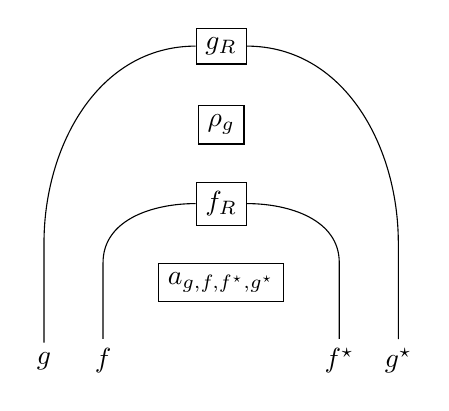
\begin{tikzpicture}
            \node[draw] (GR) {\(g_R\)};
            \node[on grid, below=1 of GR, draw] (P) {\(\rho_g\)};
            \node[on grid, below=1 of P, draw] (FR) {\(f_R\)};
            \node[on grid, below=1 of FR, draw] (A) {\(a_{g,f,\rinv f,\rinv g}\)};
            \node[on grid, below left=2cm and 2.25cm of FR] (Base1) {\(g\)};
            \node[on grid, right=0.75cm of Base1] (Base2) {\(f\)};
            \node[on grid, right=3cm of Base2] (Base3) {\(\rinv f\)};
            \node[on grid, right=0.75cm of Base3] (Base4) {\(\rinv g\)};
            \draw (Base1) to ++(0,1.5cm) to [out=90,in=180] (GR);
            \draw (Base4) to ++(0,1.5cm) to [out=90,in=0] (GR);
            \draw (Base2) to ++(0,1.25cm) to [out=90,in=180] (FR);
            \draw (Base3) to ++(0,1.25cm) to [out=90,in=0] (FR);
          \end{tikzpicture}
        \end{center}
      \item \((g \circ f)_L\) is the morphism given by the diagram
        \begin{center}
          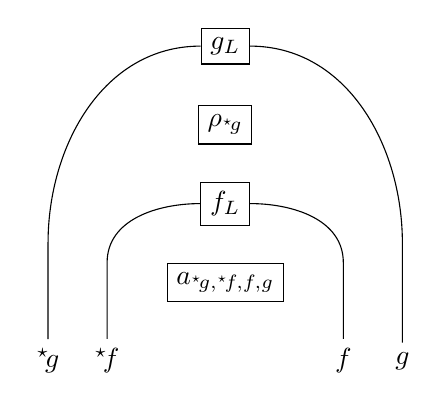
\begin{tikzpicture}
            \node[draw] (GL) {\(g_L\)};
            \node[on grid, below=1 of GL, draw] (P) {\(\rho_{\linv g}\)};
            \node[on grid, below=1 of P, draw] (FL) {\(f_L\)};
            \node[on grid, below=1 of FL, draw] {\(a_{\linv g,\linv f, f,g}\)};
            \node[on grid, below left=2cm and 2.25cm of FL] (Base1) {\(\linv g\)};
            \node[on grid, right=0.75cm of Base1] (Base2) {\(\linv f\)};
            \node[on grid, right=3cm of Base2] (Base3) {\(f\)};
            \node[on grid, right=0.75cm of Base3] (Base4) {\(g\)};
            \draw (Base1) to ++(0,1.5cm) to [out=90,in=180] (GL);
            \draw (Base4) to ++(0,1.5cm) to [out=90,in=0] (GL);
            \draw (Base2) to ++(0,1.25cm) to [out=90,in=180] (FL);
            \draw (Base3) to ++(0,1.25cm) to [out=90,in=0] (FL);
          \end{tikzpicture}
        \end{center}
      \end{itemize}

      Using both the coinductive hypothesis that \(f_L\), \(g_L\), \(f_R\),\(g_R\) are \emph{bi-invertible} and further using the other coinductive hypothesis that \emph{bi-invertibility} is preserved by both \(\circ_0\) and \(\circ_1\) for \((k'+1)\)-cells, we deduce that both \((g \circ f)_R\) and \((g \circ f)_L\) are \emph{bi-invertible} and so \(g \circ f\) is \emph{bi-invertible}.
    \item \(\alpha \circ_n \beta\) where \(n > 0\), \(\alpha: f \to g\), and \(\beta: h \to j\): Let:
      \begin{itemize}
      \item \(\rinv {(\alpha \circ_n \beta)} = \rinv \alpha \circ_n \rinv \beta\)
      \item \(\linv {(\alpha \circ_n \beta)} = \linv \alpha \circ_n \linv \beta\)
      \item Define \((\alpha \circ_n \beta)_R\) as the following composition:
        \begin{equation*}
          (\alpha \circ_n \beta) \circ (\rinv \alpha \circ_n \rinv \beta) \overset {i_{\alpha,\beta,\rinv \alpha, \rinv \beta}} \to (\alpha \circ \rinv \alpha) \circ_n (\beta \circ \rinv \beta) \overset {\alpha _R \circ_{n+1} \beta _R} \to \id_g \circ_n \id_j \to \id_{g \circ_{n-1} j}
        \end{equation*}
      \item Similarly, define \((\alpha \circ_n \beta)_L\) as the following composition:
        \begin{equation*}
          (\linv \alpha \circ_n \linv \beta) \circ (\alpha \circ_n \beta) \overset {i_{\linv \alpha, \linv \beta, \alpha, \beta}} \to (\linv \alpha \circ \alpha) \circ_n (\linv \beta \circ \beta) \overset {\alpha _L \circ_{n+1} \beta _L} \to \id_f \circ_n \id_h \to \id_{f \circ_n h}
        \end{equation*}
    \end{itemize}
    Now I claim that both \((\alpha \circ_n \beta)_R\) and \((\alpha \circ_n \beta)_L\) are both \emph{bi-invertible}. This is because these are compositions of cells that are \emph{bi-invertible} and these cells are of a higher order than \(k'\) and so we can apply the coinductive hypothesis. Hence \(\alpha \circ_n \beta\) is \emph{bi-invertible}.
  \end{itemize}
\end{proof}
A comment should be made on why this is a valid coinductive proof. Whereas inductive objects are specified by how one constructs them, coinductive objects are specified by how they are destructed. We now note that the outer coinductive hypothesis was only used for defining the coinductive part of being \emph{bi-invertible}. This means that, all that can be done with a proof that a composite is \emph{bi-invertible} is extract parts of the proof. When extracting a part of the proof we can only ``look'' finitely far into the data structure. With the observation above this means that any use of this proof will only need to use the coinductive hypothesis a finite number of times (nesting a finite amount) before using a part of the proof that does not rely on the coinductive hypothesis.

\begin{lemma}[Inverses are \emph{bi-invertible}]
  \label{lem:inverses}
  Let \(f\) be a \emph{bi-invertible} cell. Then \(\linv f\) and \(\rinv f\) are \emph{bi-invertible}.
\end{lemma}
\begin{proof}
  We show \(\rinv f\) is \emph{bi-invertible} and \(\linv f\) will follow similarly. Define the following:
  \begin{itemize}
  \item \(\rinv {(\rinv f)} = f\)
  \item \(\linv {(\rinv f)} = f\)
  \item \((\rinv f)_R: \rinv f \circ f \to \id\) is given by:
    \begin{center}
      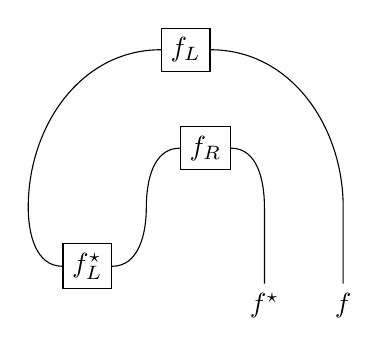
\begin{tikzpicture}
        \node (Finv) {\(\rinv f\)};
        \node [on grid, right=1cm of Finv] (F) {\(f\)};
        \node [on grid, above left=2cm and 0.75cm of Finv, draw] (FR) {\(f_R\)};
        \node [on grid, below left=1.5cm and 1.5cm of FR, draw] (FLInv) {\(\rinv {f_L}\)};
        \node [on grid, above right=2.75cm and 1.25cm of FLInv, draw] (FL) {\(f_L\)};
        \draw (Finv) to ++(0,1.25cm) to[out=90,in=0] (FR);
        \draw (FR) to[out=180,in=90] ++(-0.75cm,-0.75cm) to[out=-90,in=0] (FLInv);
        \draw (FLInv) to[out=180,in=-90] ++(-0.75cm,0.75cm) to[out=90,in=180] (FL);
        \draw (F) to ++(0,1.25cm) to[out=90,in=0] (FL);
      \end{tikzpicture}
    \end{center}
  \item \((\rinv f)_L: f \circ \rinv f \to \id\) is given by \(f_R\)
  \end{itemize}
  We get that \((\rinv f)_R\) is \emph{bi-invertible} as it is a composite of \emph{bi-invertible} morphisms (where \(\rinv {f_L}\) is \emph{bi-invertible} by coinductive hypothesis) and \((\rinv f)_L\) is trivially \emph{bi-invertible}.
\end{proof}

\begin{definition}
  We define the collection of \emph{half-adjoint invertible} morphisms coinductively as follows: For \(n > 0\), an \(n\)-cell \(f: x \to y\) is \emph{half-adjoint invertible} if:
  \begin{itemize}
  \item There exists an \(n\)-cell \(f' : y \to x\).
  \item There exists an \(n+1\)-cell \(\alpha: f \circ f' \to \id_y\).
  \item There exists an \(n+1\)-cell \(\beta: \id_x \to f' \circ f\).
  \item There exists an \(n+2\)-cell \(\gamma: (\lambda_{f'} \circ (\beta \circ_1 \id_{f'}) \circ (\id_{f'} \circ_1 \alpha) \circ \rho_{f'}) \to \id_{f'}\).
  \item \(\alpha\) is \emph{half-adjoint invertible}.
  \item \(\beta\) is \emph{half-adjoint invertible}.
  \item \(\gamma\) is \emph{half-adjoint invertible}.
  \end{itemize}

  \(\gamma\) can be graphically represented by the following diagram:
  \begin{center}
    \begin{tikzpicture}
      \node (Bottom) {\({f'}\)};
      \node[on grid, above left=1cm and 2.25cm of Bottom, draw] (Cup){\(\beta\)};
      \node[on grid, above right=2cm and 1.5cm of Cup,draw] (Cap){\(\alpha\)};
      \node[on grid, above left=1cm and 2.25cm of Cap] (Top) {\({f'}\)};
      \draw (Bottom) to++(0,2) to[out=90,in=0] (Cap);
      \draw (Cup) to[out=0,in=-90] ++(0.75,1) to[out=90,in=180] (Cap);
      \draw (Cup) to[out=180,in=-90] ++(-0.75,1) to (Top);

      \node[on grid, above right=2cm and 1cm of Bottom, font=\fontsize{20}{24}\selectfont] (Eq) {\(\Rightarrow\)};
      \node[above=0cm of Eq,font=\fontsize{15}{19}\selectfont] (Gamma) {\(\gamma\)};
      \node[on grid, right=2cm of Bottom] (L1) {\({f'}\)};
      \node[on grid, above=4cm of L1] (L2) {\({f'}\)};
      \draw (L1) to (L2);
    \end{tikzpicture}
  \end{center}
\end{definition}

\begin{theorem}
  A \emph{half-adjoint invertible} morphism is \emph{bi-invertible}.
\end{theorem}
\begin{proof}
  Suppose \(f\) is \emph{half-adjoint invertible}. Then let:
  \begin{itemize}
  \item \(\rinv f = {f'}\)
  \item \(\linv f = {f'}\)
  \item \(f_R = \alpha\)
  \item \(f_L = \rinv \beta\) (using that \(\beta\) is \emph{half-adjoint invertible} and hence \emph{bi-invertible})
  \end{itemize}
  Then by coinduction \(f_R = \alpha\) is \emph{bi-invertible} and \(\beta\) is \emph{bi-invertible} and so, by \cref{lem:inverses}, \(\rinv \beta\) is also \emph{bi-invertible} which means \(f\) is too.
\end{proof}

\begin{theorem}
  A \emph{bi-invertible} morphism is \emph{half-adjoint invertible}.
\end{theorem}
\begin{proof}
  Let \(f\) be \emph{bi-invertible}. Then let:
  \begin{itemize}
  \item \({f'} = \rinv f\)
  \item \(\alpha = f_R\)
  \item \(\beta\) is given by the following diagram:
    \begin{center}
      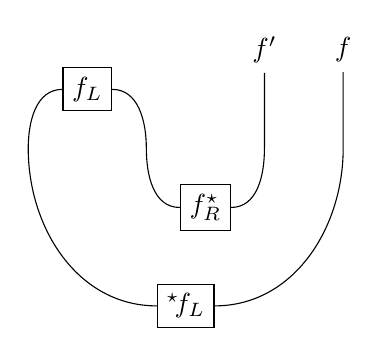
\begin{tikzpicture}
        \node (Finv) {\({f'}\)};
        \node [on grid, right=1cm of Finv] (F) {\(f\)};
        \node [on grid, below left=2cm and 0.75cm of Finv, draw] (FRInv) {\(\rinv {f_R}\)};
        \node [on grid, above left=1.5cm and 1.5cm of FRInv, draw] (FL) {\(f_L\)};
        \node [on grid, below right=2.75cm and 1.25cm of FL, draw] (FLInv) {\(\linv {f_L}\)};
        \draw (Finv) to ++(0,-1.25cm) to[out=-90,in=0] (FRInv);
        \draw (FRInv) to[out=180,in=-90] ++(-0.75cm,0.75cm) to[out=90,in=0] (FL);
        \draw (FL) to[out=180,in=90] ++(-0.75cm,-0.75cm) to[out=-90,in=180] (FLInv);
        \draw (F) to ++(0,-1.25cm) to[out=-90,in=0] (FLInv);
      \end{tikzpicture}
    \end{center}
  \item \(\gamma\) is given by the following diagram:
    \begin{center}
      \begin{tikzpicture}
        \node (G) {\({f'}\)};
        \node [on grid, below right=0.25cm and 1.75cm of G, draw] (FR) {\(f_R\)};
        \node [on grid, below right=5cm and 0.75cm of FR] (G') {\({f'}\)};
        \node [on grid, below left=3cm and 0.75cm of G, draw] (FRInv) {\(\rinv {(f_R)}\)};
        \node [on grid, above left=1.5cm and 1.5cm of FRInv, draw] (FL) {\(f_L\)};
        \node [on grid, below right=2.75cm and 1.25cm of FL, draw] (FLInv) {\(\linv {(f_L)}\)};
        \draw (G) to ++(0,-2.25cm) to[out=-90,in=0] (FRInv);
        \draw (FRInv) to[out=180,in=-90] ++(-0.75cm,0.75cm) to[out=90,in=0] (FL);
        \draw (FL) to[out=180,in=90] ++(-0.75cm,-0.75cm) to[out=-90,in=180] (FLInv);
        \draw (FR) to[out=180,in=90] ++(-0.75cm,-0.75cm) to ++(0,-1.25cm) to[out=-90,in=0] (FLInv);
        \draw (FR) to[out=0,in=90] ++(0.75cm,-0.75cm) to (G');

        \node [on grid, below right=2.75cm and 3.75cm of G,font=\fontsize{20}{24}\selectfont] (A1) {\(\Rightarrow\)};
        \node [on grid, above=0.5cm of A1] (A1Text) {isotopy};

        \node [on grid, right=8cm of G] (G1) {\({f'}\)};
        \node [on grid, below left=2cm and 0.75cm of G1, draw] (FRInv1) {\(\rinv {(f_R)}\)};
        \node [on grid, below=1cm of FRInv1, draw] (FR1) {\(f_R\)};
        \node [on grid, above left=1.5cm and 1.5cm of FRInv1, draw] (FL1) {\(f_L\)};
        \node [on grid, below left=1.5cm and 1.5cm of FR1, draw] (FLInv1) {\(\linv {(f_L)}\)};
        \node [on grid, below right=2cm and 0.75cm of FR1] (G'1) {\({f'}\)};
        \draw (G1) to ++(0,-1.25cm) to[out=-90,in=0] (FRInv1);
        \draw (FRInv1) to[out=180,in=-90] ++(-0.75cm,0.75cm) to[out=90,in=0] (FL1);
        \draw (FL1) to[out=180,in=90] ++(-0.75cm,-0.75cm) to ++(0,-2.5cm) to[out=-90,in=180] (FLInv1);
        \draw (FR1) to[out=180,in=90] ++(-0.75cm,-0.75cm) to[out=-90,in=0] (FLInv1);
        \draw (FR1) to[out=0,in=90] ++(0.75cm,-0.75cm) to (G'1);

        \node [on grid, rotate=-90, below left=1.5cm and 1.5cm of G'1,font=\fontsize{20}{24}\selectfont] (A2) {\(\Rightarrow\)};
        \node [on grid, left=1cm of A2] (A2Text) {\((f_R)_R\)};

        \node [on grid, below=8cm of G1] (G2) {\({f'}\)};
        \node [on grid, below=3.5cm of G2] (G'2) {\({f'}\)};
        \node [on grid, below left=1cm and 2.25cm of G2, draw] (FL2) {\(f_L\)};
        \node [on grid, below=1.5cm of FL2, draw] (FLInv2) {\(\linv {(f_L)}\)};
        \draw (G2) to (G'2);
        \draw (FL2) to[out=0,in=90] ++(0.75cm,-0.75cm) to[out=-90,in=0] (FLInv2);
        \draw (FL2) to[out=180,in=90] ++(-0.75cm,-0.75cm) to[out=-90,in=180] (FLInv2);

        \node [on grid, below left=0.75cm and 2.5cm of FL2,font=\fontsize{20}{24}\selectfont] (A3) {\(\Leftarrow\)};
        \node [on grid, above=0.5cm of A3] (A3Text) {\((f_L)_L\)};

        \node [on grid, below=8cm of G] (G3) {\({f'}\)};
        \node [on grid, below=3.5cm of G3] (G'3) {\({f'}\)};
        \draw (G3) to (G'3);
      \end{tikzpicture}
    \end{center}
    \(\alpha\) is \emph{bi-invertible}. \(\beta\) is a composite of \emph{bi-invertible} morphisms and inverses of \emph{bi-invertible} morphisms so is itself \emph{bi-invertible}. \(\gamma\) consists of a composition of \emph{bi-invertible} morphisms and isotopies so is \emph{bi-invertible}. Therefore all of these are \emph{half-adjoint invertible} by coinduction and so \(f\) is \emph{half-adjoint invertible}.
  \end{itemize}
\end{proof}
\end{document}